%%
%% This is file `sample-sigplan.tex',
%% generated with the docstrip utility.
%%
%% The original source files were:
%%
%% samples.dtx  (with options: `all,proceedings,bibtex,sigplan')
%% 
%% IMPORTANT NOTICE:
%% 
%% For the copyright see the source file.
%% 
%% Any modified versions of this file must be renamed
%% with new filenames distinct from sample-sigplan.tex.
%% 
%% For distribution of the original source see the terms
%% for copying and modification in the file samples.dtx.
%% 
%% This generated file may be distributed as long as the
%% original source files, as listed above, are part of the
%% same distribution. (The sources need not necessarily be
%% in the same archive or directory.)
%%
%%
%% Commands for TeXCount
%TC:macro \cite [option:text,text]
%TC:macro \citep [option:text,text]
%TC:macro \citet [option:text,text]
%TC:envir table 0 1
%TC:envir table* 0 1
%TC:envir tabular [ignore] word
%TC:envir displaymath 0 word
%TC:envir math 0 word
%TC:envir comment 0 0
%%
%%
%% The first command in your LaTeX source must be the \documentclass
%% command.
%%
%% For submission and review of your manuscript please change the
%% command to \documentclass[manuscript, screen, review]{acmart}.
%%
%% When submitting camera ready or to TAPS, please change the command
%% to \documentclass[sigconf]{acmart} or whichever template is required
%% for your publication.
%%
%%
\documentclass[sigplan,screen]{acmart}

%%
%% \BibTeX command to typeset BibTeX logo in the docs
\AtBeginDocument{%
  \providecommand\BibTeX{{%
    Bib\TeX}}}

%% Rights management information.  This information is sent to you
%% when you complete the rights form.  These commands have SAMPLE
%% values in them; it is your responsibility as an author to replace
%% the commands and values with those provided to you when you
%% complete the rights form.
\setcopyright{acmlicensed}
\copyrightyear{2024}
\acmYear{2018}
\acmDOI{XXXXXXX.XXXXXXX}

%% These commands are for a PROCEEDINGS abstract or paper.
\acmConference[Cloud computing e infraestructura para Big Data]{Make sure to enter the correct
  conference title from your rights confirmation emai}{Agosto 31-08,
  2024}{Santa Cruz, Bolivia}
%%
%%  Uncomment \acmBooktitle if the title of the proceedings is different
%%  from ``Proceedings of ...''!
%%
%%\acmBooktitle{Woodstock '18: ACM Symposium on Neural Gaze Detection,
%%  June 03--05, 2018, Woodstock, NY}
\acmISBN{978-1-4503-XXXX-X/18/06}


%%
%% Submission ID.
%% Use this when submitting an article to a sponsored event. You'll
%% receive a unique submission ID from the organizers
%% of the event, and this ID should be used as the parameter to this command.
%%\acmSubmissionID{123-A56-BU3}

%%
%% For managing citations, it is recommended to use bibliography
%% files in BibTeX format.
%%
%% You can then either use BibTeX with the ACM-Reference-Format style,
%% or BibLaTeX with the acmnumeric or acmauthoryear sytles, that include
%% support for advanced citation of software artefact from the
%% biblatex-software package, also separately available on CTAN.
%%
%% Look at the sample-*-biblatex.tex files for templates showcasing
%% the biblatex styles.
%%

%%
%% The majority of ACM publications use numbered citations and
%% references.  The command \citestyle{authoryear} switches to the
%% "author year" style.
%%
%% If you are preparing content for an event
%% sponsored by ACM SIGGRAPH, you must use the "author year" style of
%% citations and references.
%% Uncommenting
%% the next command will enable that style.
%%\citestyle{acmauthoryear}
\usepackage{tabularx}
\usepackage{graphicx}
\usepackage[spanish]{babel}

\newcommand{\staricon}[1]{
    \begin{tikzpicture}[scale=#1]
        \filldraw[fill=yellow, draw=black] 
        (0,0) -- (0.2,0.6) -- (0.6,0.6) -- (0.3,0.9) -- (0.4,1.4) -- (0,1.1) -- (-0.4,1.4) -- (-0.3,0.9) -- (-0.6,0.6) -- (-0.2,0.6) -- cycle;
    \end{tikzpicture}
}

%%
%% end of the preamble, start of the body of the document source.
\begin{document}

%%
%% The "title" command has an optional parameter,
%% allowing the author to define a "short title" to be used in page headers.
\title{Api Gateway: Kong vs. AWS}

%%
%% The "author" command and its associated commands are used to define
%% the authors and their affiliations.
%% Of note is the shared affiliation of the first two authors, and the
%% "authornote" and "authornotemark" commands
%% used to denote shared contribution to the research.
\author{Bravo Peña}
\author{Darlyn}
\affiliation{
  \institution{UAGRM}
  \city{Santa Cruz}
  \country{Bolivia}
}
\email{contact@bpdarlyn.com}

\author{Torrejón Mendez}
\author{Joel Gabriel}
\affiliation{
  \institution{UAGRM}
  \city{Santa Cruz}
  \country{Bolivia}
}
\email{joel.torrejon.mendez@gmail.com}

\author{Valle Tamayo}
\author{Brandon Jason}
\affiliation{
  \institution{UAGRM}
  \city{Santa Cruz}
  \country{Bolivia}}
\email{bjvtamayo78@gmail.com}
%%
%% By default, the full list of authors will be used in the page
%% headers. Often, this list is too long, and will overlap
%% other information printed in the page headers. This command allows
%% the author to define a more concise list
%% of authors' names for this purpose.
\renewcommand{\shortauthors}{Bravo - Torrejón - Valle}

%%
%% The code below is generated by the tool at http://dl.acm.org/ccs.cfm.
%% Please copy and paste the code instead of the example below.
%%
% \begin{CCSXML}
% <ccs2012>
%  <concept>
%   <concept_id>00000000.0000000.0000000</concept_id>
%   <concept_desc>Do Not Use This Code, Generate the Correct Terms for Your Paper</concept_desc>
%   <concept_significance>500</concept_significance>
%  </concept>
%  <concept>
%   <concept_id>00000000.00000000.00000000</concept_id>
%   <concept_desc>Do Not Use This Code, Generate the Correct Terms for Your Paper</concept_desc>
%   <concept_significance>300</concept_significance>
%  </concept>
%  <concept>
%   <concept_id>00000000.00000000.00000000</concept_id>
%   <concept_desc>Do Not Use This Code, Generate the Correct Terms for Your Paper</concept_desc>
%   <concept_significance>100</concept_significance>
%  </concept>
%  <concept>
%   <concept_id>00000000.00000000.00000000</concept_id>
%   <concept_desc>Do Not Use This Code, Generate the Correct Terms for Your Paper</concept_desc>
%   <concept_significance>100</concept_significance>
%  </concept>
% </ccs2012>
% \end{CCSXML}

% \ccsdesc[500]{Do Not Use This Code~Generate the Correct Terms for Your Paper}
% \ccsdesc[300]{Do Not Use This Code~Generate the Correct Terms for Your Paper}
% \ccsdesc{Do Not Use This Code~Generate the Correct Terms for Your Paper}
% \ccsdesc[100]{Do Not Use This Code~Generate the Correct Terms for Your Paper}

%%
%% Keywords. The author(s) should pick words that accurately describe
%% the work being presented. Separate the keywords with commas.
% \keywords{Do, Not, Us, This, Code, Put, the, Correct, Terms, for,
%   Your, Paper}
%% A "teaser" image appears between the author and affiliation
%% information and the body of the document, and typically spans the
%% page.
\begin{teaserfigure}
  
\includegraphics[width=\textwidth]{images/logo_soe.png}
  \Description{Enjoying the baseball game from the third-base
  seats. Ichiro Suzuki preparing to bat.}
  \label{fig:teaser}
\end{teaserfigure}

\received{20 February 2007}
\received[revised]{12 March 2009}
\received[accepted]{5 June 2009}

%%
%% This command processes the author and affiliation and title
%% information and builds the first part of the formatted document.
\maketitle

% Document content
\section{Introducción}
ACM's consolidated article template, introduced in 2017, provides a
consistent \LaTeX\ style for use across ACM publications, and
incorporates accessibility and metadata-extraction functionality
necessary for future Digital Library endeavors. Numerous ACM and
SIG-specific \LaTeX\ templates have been examined, and their unique
features\cite{ibm-sl} incorporated into this single new template.

If you are new to publishing with ACM, this document is a valuable
guide to the process of preparing your work for publication. If you
have published with ACM before, this document provides insight and
instruction into more \cite{ibm-ml} recent changes to the article template.

The ``\verb|acmart|'' document class can be used to prepare articles
for any ACM publication --- conference or journal, and for any stage
of publication, from\cite{ibm-usl} review to final ``camera-ready'' copy, to the
author's own version, with {\itshape very} few changes to the source.

\section{Api Gateway}
As noted in the introduction, the ``\verb|acmart|'' document class can
be used to prepare many different kinds of documentation --- a
double-anonymous initial submission of a full-length technical paper, a
two-page SIGGRAPH Emerging Technologies abstract, a ``camera-ready''
journal article, a SIGCHI Extended Abstract, and more --- all by
selecting the appropriate {\itshape template style} and {\itshape
  template parameters}.

This document will explain the major features of the document
class. For further information, the {\itshape \LaTeX\ User's Guide} is
available from
\url{https://www.acm.org/publications/proceedings-template}.

\subsection{Template Styles}

The primary parameter given to the ``\verb|acmart|'' document class is
the {\itshape template style} which corresponds to the kind of publication
or SIG publishing the work. This parameter is enclosed in square
brackets and is a part of the {\verb|documentclass|} command:
\begin{verbatim}
  \documentclass[STYLE]{acmart}
\end{verbatim}

Journals use one of three template styles. All but three ACM journals
use the {\verb|acmsmall|} template style:
\begin{itemize}
\item {\texttt{acmsmall}}: The default journal template style.
\item {\texttt{acmlarge}}: Used by JOCCH and TAP.
\item {\texttt{acmtog}}: Used by TOG.
\end{itemize}

The majority of conference proceedings documentation will use the {\verb|acmconf|} template style.
\begin{itemize}
\item {\texttt{sigconf}}: The default proceedings template style.
\item{\texttt{sigchi}}: Used for SIGCHI conference articles.
\item{\texttt{sigplan}}: Used for SIGPLAN conference articles.
\end{itemize}

\subsection{Template Parameters}

In addition to specifying the {\itshape template style} to be used in
formatting your work, there are a number of {\itshape template parameters}
which modify some part of the applied template style. A complete list
of these parameters can be found in the {\itshape \LaTeX\ User's Guide.}

Frequently-used parameters, or combinations of parameters, include:
\begin{itemize}
\item {\texttt{anonymous,review}}: Suitable for a ``double-anonymous''
  conference submission. Anonymizes the work and includes line
  numbers. Use with the \texttt{\acmSubmissionID} command to print the
  submission's unique ID on each page of the work.
\item{\texttt{authorversion}}: Produces a version of the work suitable
  for posting by the author.
\item{\texttt{screen}}: Produces colored hyperlinks.
\end{itemize}

This document uses the following string as the first command in the
source file:
\begin{verbatim}
\documentclass[sigplan,screen]{acmart}
\end{verbatim}

\section{Kong}
As noted in the introduction, the ``\verb|acmart|'' document class can
be used to prepare many different kinds of documentation --- a
double-anonymous initial submission of a full-length technical paper, a
two-page SIGGRAPH Emerging Technologies abstract, a ``camera-ready''
journal article, a SIGCHI Extended Abstract, and more --- all by
selecting the appropriate {\itshape template style} and {\itshape
  template parameters}.

This document will explain the major features of the document
class. For further information, the {\itshape \LaTeX\ User's Guide} is
available from
\url{https://www.acm.org/publications/proceedings-template}.

\subsection{Template Styles}

The primary parameter given to the ``\verb|acmart|'' document class is
the {\itshape template style} which corresponds to the kind of publication
or SIG publishing the work. This parameter is enclosed in square
brackets and is a part of the {\verb|documentclass|} command:
\begin{verbatim}
  \documentclass[STYLE]{acmart}
\end{verbatim}

Journals use one of three template styles. All but three ACM journals
use the {\verb|acmsmall|} template style:
\begin{itemize}
\item {\texttt{acmsmall}}: The default journal template style.
\item {\texttt{acmlarge}}: Used by JOCCH and TAP.
\item {\texttt{acmtog}}: Used by TOG.
\end{itemize}

The majority of conference proceedings documentation will use the {\verb|acmconf|} template style.
\begin{itemize}
\item {\texttt{sigconf}}: The default proceedings template style.
\item{\texttt{sigchi}}: Used for SIGCHI conference articles.
\item{\texttt{sigplan}}: Used for SIGPLAN conference articles.
\end{itemize}

\subsection{Template Parameters}

In addition to specifying the {\itshape template style} to be used in
formatting your work, there are a number of {\itshape template parameters}
which modify some part of the applied template style. A complete list
of these parameters can be found in the {\itshape \LaTeX\ User's Guide.}

Frequently-used parameters, or combinations of parameters, include:
\begin{itemize}
\item {\texttt{anonymous,review}}: Suitable for a ``double-anonymous''
  conference submission. Anonymizes the work and includes line
  numbers. Use with the \texttt{\acmSubmissionID} command to print the
  submission's unique ID on each page of the work.
\item{\texttt{authorversion}}: Produces a version of the work suitable
  for posting by the author.
\item{\texttt{screen}}: Produces colored hyperlinks.
\end{itemize}

This document uses the following string as the first command in the
source file:
\begin{verbatim}
\documentclass[sigplan,screen]{acmart}
\end{verbatim}

\section{Amazon API Gateway}

Amazon API Gateway \cite{aws-api-gateway-docs} es un servicio que ofrece claves fundamentales que todo API Gateway debería tener: \
\begin{itemize}
	\item Único punto de entrada
	\item Conductor de Rutas
	\item Protocolo de transformación
	\item Registry and Discovery
	\item Autenticación y Autorización
	\item Escalabilidad y Orquestación
	\item Thortting (Limites)
	\item Monitorización
\end{itemize}

Pero tiene características adicionales como : \

\begin{itemize}
	\item Son basadas en HTTP
	\item Son basadas en websockets
	\item Forma parte de un set de infraestructura llamada serverless (pay as you go)
\end{itemize}
\subsection{Arquitectura}
\begin{figure}[htbp]
	\centering
	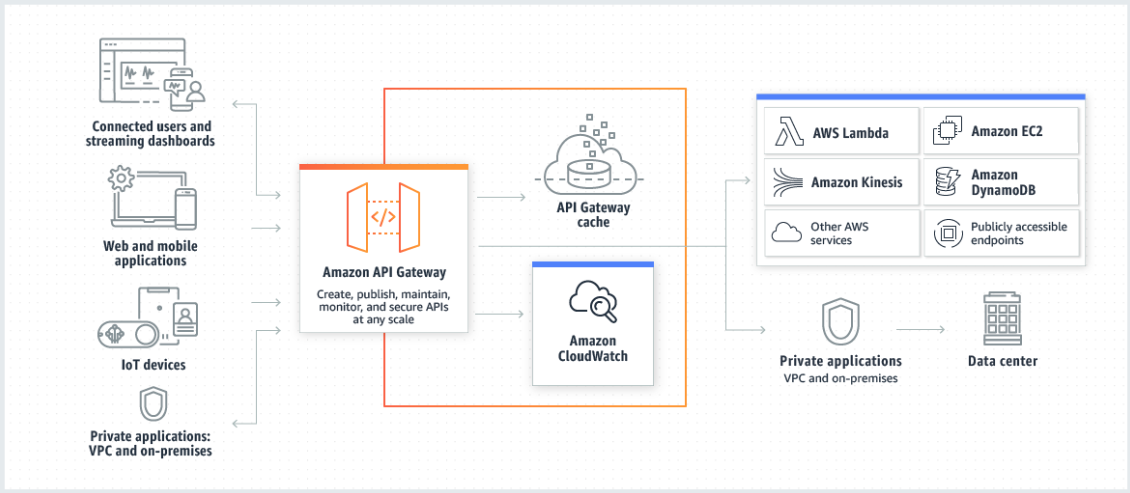
\includegraphics[width=\columnwidth]{images/architecture_aws_api_gateway}
	\caption{Arquitectura general de Aws API Gateway}
	\label{fig:architecture_aws_api_gateway}
\end{figure}

\subsection{Autenticación}
A pesar de ser un servicio de paga su autenticación es muy flexible porque te permite usar un proveedor existente de AWS tales como: AWS Identity, Access Management policies, Lambda authorizer y Amazon Cognito

\subsection{Tipos de Endpoints}
Amazon ofrece 2 tipos de Endpoints más usados:
\subsubsection{Edge Optimized API endpoints}
Las solicitudes se enrutan al Cloudfront más cercano, Point of Presence(POP). El cuál ayuda si tus clientes están distribuídos geográficamente, cuando creas un API Gateway y mantienes muchos de los parámetros por defecto no necesitas configurar esta opción ya que es el comportamiento predeterminado.

\subsubsection{Tipo de Endpoint Regional}
Especial para clientes en la misma región, por ejemplo cuando algún cliente que tiene una instancia de EC2 llama una api que también se encuentra en la misma región o también cuando necesitas baja latencia o respuesta rápida, al limitar la comunicación dentro de una región se minimiza las latencias y los costos asociados a la red.

\subsection{Integraciones}
Una vez que se define un API Method (POST, PUT, DELETE, ETC) tu necesitas definir un backend endpoint que puede ser cualquiera de:\
\begin{itemize}
	\item Ejecutar un Service Action como: SQS, STEPFUNCTION
	\item Función \textbf{Lambda}
	\item Otro \textbf{HTTP Endpoint}
\end{itemize}

Para la comunicación con el backend tu necesitas definir: \

\begin{description}
	\item[Integration Request:] Como quieres formatear la solicitud para posteriormente enviar la request formateada a tu backend
	\item[Integration Response:] Cómo quieres formatear la respuesta del backend para ser respondida al client.
\end{description}

\subsection{Validaciones}
Puedes definir validaciones antes de ejecutar tu backend, reduciendo ejecuciones innecesarias en tu backend, ya que api gateway puede retornar un error 400 al cliente sin pasar por el backend.

\subsection{Transformaciones de Data}
Te permite trasformar tu data, usando un motor de expresiones tu puedes cambiar, los headers, query arguments, body usando \textbf{mapping templates}.

\subsection{OpenApi}
Si ya tenías o usas OpenApi para definir tus endpoints puedes continuar haciendolo y agregar algunos campos adicionales para desplegar estos endpoints en API Gateway sin necesidad de definirlos de forma manual o usando IAAC.
De momento solo ofrece soporte para \textbf{OpenApi v2.0} y \textbf{OpenApi v3.0}
\subsection{Seguridad}
puedes configurar solicitudes cruzadas por endpoint (api method). También debido a que AWS tiene habilitado de forma predeterminada la detección de ataques de RED como un DOS estas siendo protegido también por toda la estructura de AWS.

\subsection{Compartir Endpoints a tus Clientes}
Puedes configurar API Keys para tus clientes y también puedes configurar También definir cuotas por API que tus clientes pueden usar así como el throttling que tus customers deben tener y si sobre pasa de estos límites Api Gateway rechazará automáticamente la solicitud.

\subsection{Monitorización}
Tienes innumerables métricas diseñadas por AWS, puedes también hacer uso de Cloudwatch logs y X-Ray. Además que en los mismos servicios puedes subscribirte a métricas y recibiendo alarmas de los eventos que 
\section{Benchmark}

Authors of any work published by ACM will need to complete a rights
form. Depending on the kind of work, and the rights management choice
made by the author, this may be copyright transfer, permission,
license, or an OA (open access) agreement.

Regardless of the rights management choice, the author will receive a
copy of the completed rights form once it has been submitted. This
form contains \LaTeX\ commands that must be copied into the source
document. When the document source is compiled, these commands and
their parameters add formatted text to several areas of the final
document:
\begin{itemize}
\item the ``ACM Reference Format'' text on the first page.
\item the ``rights management'' text on the first page.
\item the conference information in the page header(s).
\end{itemize}

Rights information is unique to the work; if you are preparing several
works for an event, make sure to use the correct set of commands with
each of the works.

The ACM Reference Format text is required for all articles over one
page in length, and is optional for one-page articles (abstracts).

\newpage
\section{Conclusión}

The ``\verb|figure|'' environment should be used for figures. One or
more images can be placed within a figure. If your figure contains
third-party material, you must clearly identify it as such, as shown
in the example below.
\begin{figure}[h]
  \centering
  
\includegraphics[width=\linewidth]{images/banner}
  \caption{1907 Franklin Model D roadster. Photograph by Harris \&
    Ewing, Inc. [Public domain], via Wikimedia
    Commons. (\url{https://goo.gl/VLCRBB}).}
  \Description{A woman and a girl in white dresses sit in an open car.}
\end{figure}

Your figures should contain a caption which describes the figure to
the reader.

Figure captions are placed {\itshape below} the figure.

Every figure should also have a figure description unless it is purely
decorative. These descriptions convey what’s in the image to someone
who cannot see it. They are also used by search engine crawlers for
indexing images, and when images cannot be loaded.

A figure description must be unformatted plain text less than 2000
characters long (including spaces).  {\bfseries Figure descriptions
  should not repeat the figure caption – their purpose is to capture
  important information that is not already provided in the caption or
  the main text of the paper.} For figures that convey important and
complex new information, a short text description may not be
adequate. More complex alternative descriptions can be placed in an
appendix and referenced in a short figure description. For example,
provide a data table capturing the information in a bar chart, or a
structured list representing a graph.  For additional information
regarding how best to write figure descriptions and why doing this is
so important, please see
\url{https://www.acm.org/publications/taps/describing-figures/}.

\subsection{The ``Teaser Figure''}

A ``teaser figure'' is an image, or set of images in one figure, that
are placed after all author and affiliation information, and before
the body of the article, spanning the page. If you wish to have such a
figure in your article, place the command immediately before the
\verb|\maketitle| command:
\begin{verbatim}
  \begin{teaserfigure}
    \includegraphics[width=\textwidth]{sampleteaser}
    \caption{figure caption}
    \Description{figure description}
  \end{teaserfigure}
\end{verbatim}


%%
%% The acknowledgments section is defined using the "acks" environment
%% (and NOT an unnumbered section). This ensures the proper
%% identification of the section in the article metadata, and the
%% consistent spelling of the heading.
% \begin{acks}
% To Robert, for the bagels and explaining CMYK and color spaces.
% \end{acks}

%%
%% The next two lines define the bibliography style to be used, and
%% the bibliography file.
\bibliographystyle{ACM-Reference-Format}
\bibliography{bibliography}


%%
%% If your work has an appendix, this is the place to put it.
\appendix

\end{document}
\endinput
%%
%% End of file `sample-sigplan.tex'.